\chapter{Developer Survey}

\section*{Survey questions}
The survey given to Dwolla developers (Chapter~\ref{sec:survey}) is presented in Figure~\ref{fig:surveyPDF1} and Figure~\ref{fig:surveyPDF2}.

\begin{figure}[h]
   \centering
   \begin{tabular}{@{}c@{\hspace{.2cm}}c@{}}
       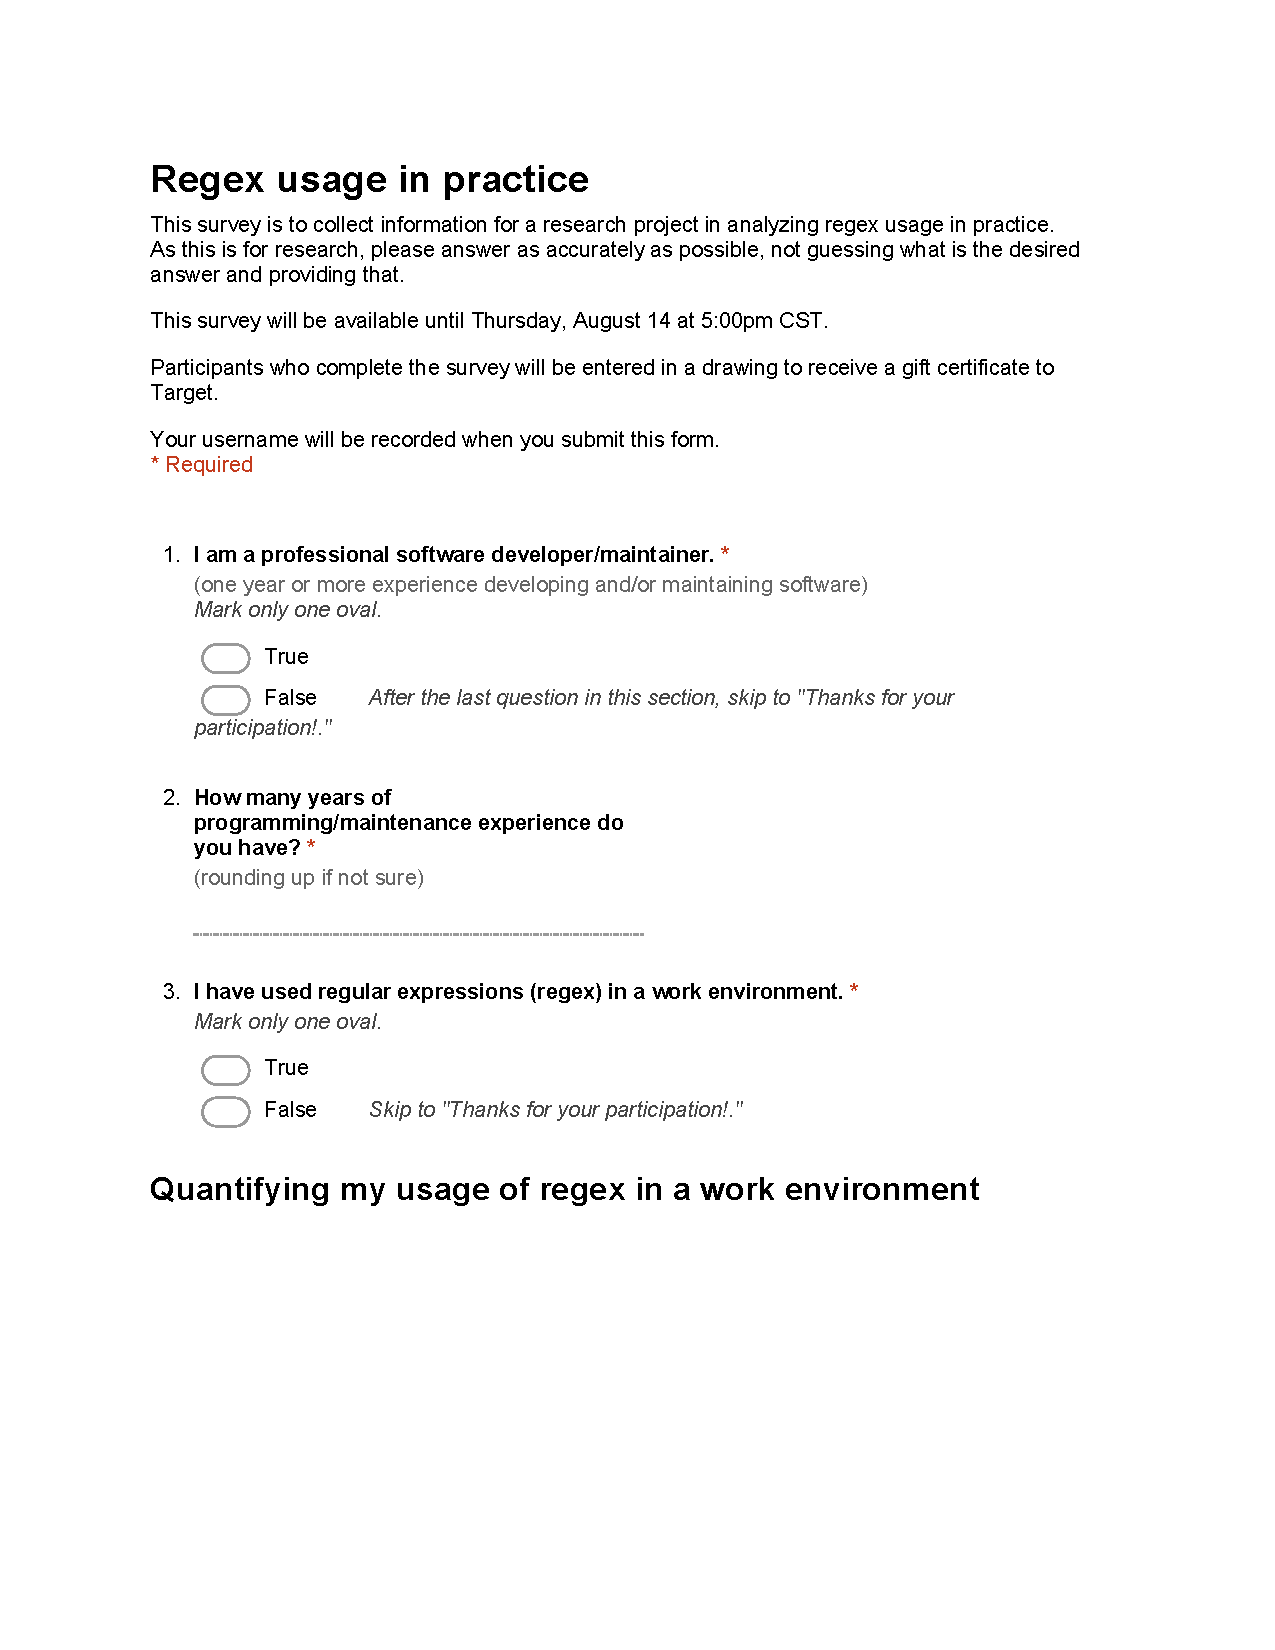
\includegraphics[page=1,width=.5\textwidth]{nontex/appendix/regexUsageInPracticeSurvey} &
       \includegraphics[page=2,width=.5\textwidth]{nontex/appendix/regexUsageInPracticeSurvey} \\[.2cm]
       \includegraphics[page=3,width=.5\textwidth]{nontex/appendix/regexUsageInPracticeSurvey} &
       \includegraphics[page=4,width=.5\textwidth]{nontex/appendix/regexUsageInPracticeSurvey} \\[.2cm]
   \end{tabular}
 \caption{Pages 1-4 (of 8) from the survey deployed to professional developers}
 \label{fig:surveyPDF1}
\end{figure}


\begin{figure}[h]
   \centering
   \begin{tabular}{@{}c@{\hspace{.2cm}}c@{}}
       \includegraphics[page=5,width=.5\textwidth]{nontex/appendix/regexUsageInPracticeSurvey} &
       \includegraphics[page=6,width=.5\textwidth]{nontex/appendix/regexUsageInPracticeSurvey} \\[.2cm]
       \includegraphics[page=7,width=.5\textwidth]{nontex/appendix/regexUsageInPracticeSurvey} &
       \includegraphics[page=8,width=.5\textwidth]{nontex/appendix/regexUsageInPracticeSurvey} \\[.2cm]
   \end{tabular}
 \caption{Pages 5-8 (of 8) from the survey deployed to professional developers}
 \label{fig:surveyPDF2}
\end{figure}

\section*{Survey Responses}
This section contains the responses to survey questions, grouped by common theme.
\begin{table}
\centering
\begin{tabular}{|c|c|c|c|}
\hline
 & I am a dev. & years experience & I have used regex at work\\
\noalign{\hrule height 0.08em}
A & true & 1 & true\\
\hline
B & false & 1 & false\\
\hline
C & true & 3 & true\\
\hline
D & true & 5 & true\\
\hline
E & false & 5 & false\\
\hline
F & true & 6 & true\\
\hline
G & true & 6 & true\\
\hline
H & true & 7 & true\\
\hline
I & true & 7 & true\\
\hline
J & true & 8 & true\\
\hline
K & true & 8 & true\\
\hline
L & true & 9 & true\\
\hline
M & true & 9 & true\\
\hline
N & true & 10 & true\\
\hline
O & true & 10 & true\\
\hline
P & true & 12 & true\\
\hline
Q & true & 15 & true\\
\hline
R & true & 15 & true\\
\hline
S & true & 15 & true\\
\hline
T & true & 16 & true\\
\noalign{\hrule height 0.08em}
\end{tabular}
\label{table:surveyQ01T3}
\caption{\small{Qualifying questions Q1: I am a professional software developer/maintainer.  and Q3: I have used regular expressions (regex) in a work environment.  If response is false to Q1 or Q3, then the survey is complete for that respondent.  Q2: How many years of programming/maintenance experience do you have?}}
\end{table}


\begin{table}[!htbp]
\centering
\begin{tabular}{|c|c|c|c|c|c|c|}

 & General purpose & scripting & query languages & command line & text editor & other\\
\noalign{\hrule height 0.08em}
A & 51-100 & 101+ & 21-50 & 101+ & 51-100 & 0\\
\hline
B &  &  &  &  &  & \\
\hline
C & 11-20 & 21-50 & 0 & 51-100 & 51-100 & 0\\
\hline
D & 0 & 21-50 & 0 & 51-100 & 101+ & 0\\
\hline
E &  &  &  &  &  & \\
\hline
F & 1-5 & 1-5 & 1-5 & 1-5 & 1-5 & 0\\
\hline
G & 6-10 & 0 & 0 & 6-10 & 11-20 & 0\\
\hline
H & 1-5 & 0 & 1-5 & 1-5 & 1-5 & 0\\
\hline
I & 1-5 & 11-20 & 0 & 6-10 & 11-20 & 0\\
\hline
J & 1-5 & 1-5 & 0 & 101+ & 101+ & 0\\
\hline
K & 11-20 & 11-20 & 0 & 101+ & 101+ & 0\\
\hline
L & 21-50 & 1-5 & 0 & 1-5 & 1-5 & 0\\
\hline
M & 6-10 & 0 & 0 & 11-20 & 11-20 & 0\\
\hline
N & 6-10 & 6-10 & 0 & 1-5 & 1-5 & 0\\
\hline
O & 1-5 & 0 & 0 & 0 & 0 & 0\\
\hline
P & 101+ & 6-10 & 0 & 51-100 & 21-50 & 0\\
\hline
Q & 6-10 & 6-10 & 0 & 1-5 & 1-5 & 0\\
\hline
R & 1-5 & 1-5 & 0 & 6-10 & 0 & 21-50\\
\hline
S & 11-20 & 11-20 & 0 & 11-20 & 11-20 & 0\\
\hline
T & 6-10 & 0 & 0 & 0 & 11-20 & 0\\
\noalign{\hrule height 0.08em}
101+ & 1 & 1 & 0 & 3 & 3 & 0\\
\hline
51-100 & 1 & 0 & 0 & 3 & 2 & 0\\
\hline
21-50 & 1 & 2 & 1 & 0 & 1 & 1\\
\hline
11-20 & 3 & 3 & 0 & 2 & 5 & 0\\
\hline
6-10 & 5 & 3 & 0 & 3 & 0 & 0\\
\hline
1-5 & 6 & 4 & 2 & 5 & 5 & 0\\
\hline
0 & 1 & 5 & 15 & 2 & 5 & 0\\
\hline
\end{tabular}
\label{table:surveyQ04}
\caption{\small{Q4: Please estimate the N regex you compose per year (by technical environment). }}
\end{table}


\begin{table}[!htbp]
\centering
\begin{tiny}
\label{table:surveyQ05}
\caption{\small{Q5: Please describe how often you compose regex for a particular problem type. }}
\begin{tabular}{|c|c|c|c|c|c|c|c|c|c|}
\hline
 & \textbf{Capturing} & \begin{minipage}{0.5in}\textbf{Counting Lines}\end{minipage} & \begin{minipage}{0.5in}\textbf{Counting All}\end{minipage} & \textbf{Finding} & \textbf{Filtering} & \textbf{Single Char} & \begin{minipage}{0.6in}\textbf{Parse User Input}\end{minipage} & \begin{minipage}{0.6in}\textbf{Parse Generated} \end{minipage}& \textbf{Other} \\
\noalign{\hrule height 0.08em}
v. freq & 1 & 1 & 1 & 3 & 0 & 0 & 2 & 2 & 0\\
\hline
freq. & 9 & 2 & 3 & 7 & 1 & 0 & 5 & 1 & 1\\
\hline
occ. & 3 & 5 & 4 & 3 & 8 & 1 & 5 & 4 & 0\\
\hline
rarely & 5 & 3 & 3 & 4 & 2 & 3 & 3 & 3 & 0\\
\hline
v. rarely & 0 & 3 & 4 & 1 & 5 & 5 & 3 & 5 & 1\\
\hline
never & 0 & 4 & 3 & 0 & 2 & 9 & 0 & 3 & 16\\
\hline
 & 3.3 & 2.0 & 2.2 & 3.4 & 2.1 & 0.8 & 3 & 2.1 & 0.3\\
\noalign{\hrule height 0.08em}
\end{tabular}
\end{tiny}
\end{table}


\paragraph{Responses to Q6} Question six~\ref{table:surveyQ06} may be hard to understand by itself and is mostly empty.  An explanation is provided here.  Two participants responded to question 6.
User A indicated `Javascript', although they did not indicate an `other' choice besides the default.  User R indicated `Matchers for cucumber test fixtures', referring to 21-50 `other' regexes composed per year and `frequently' composing for other  purposes.

\begin{table}
\centering
\begin{tabular}{|c|c|}
& why was `other' indicated in Q4 or Q5? \\
\noalign{\hrule height 0.08em}
A & Javascript\\
\hline
B & \\
\hline
C & \\
\hline
D & \\
\hline
E & \\
\hline
F & \\
\hline
G & \\
\hline
H & \\
\hline
I & \\
\hline
J & \\
\hline
K & \\
\hline
L & \\
\hline
M & \\
\hline
N & \\
\hline
O & \\
\hline
P & \\
\hline
Q & \\
\hline
R & Matchers for cucumber test fixtures\\
\hline
S & \\
\hline
T & \\
\noalign{\hrule height 0.08em}
\end{tabular}
\label{table:surveyQ06}
\caption{\small{Q6: If you selected 'other' in either or both of the above 2 questions, please explain below what you are indicating}}
\end{table}


\begin{table}
\centering
\begin{tabular}{|c|c|c|}
\noalign{\hrule height 0.04em}
 & N regex per year & N days without using regex\\
\noalign{\hrule height 0.08em}
A & 500 & 2\\
\hline
B &  & \\
\hline
C & 200 & 14\\
\hline
D & 200 & 2\\
\hline
E &  & \\
\hline
F & 5 & 60\\
\hline
G & 10 & 150\\
\hline
H & 3 & 14\\
\hline
I & 100 & 7\\
\hline
J & 220 & 6\\
\hline
K & 1000 & 14\\
\hline
L & 50 & 7\\
\hline
M & 60 & 7\\
\hline
N & 25 & 120\\
\hline
O & 4 & 90\\
\hline
P & 400 & 2\\
\hline
Q & 20 & 30\\
\hline
R & 200 & 30\\
\hline
S & 70 & 3\\
\hline
T & 30 & 3\\
\noalign{\hrule height 0.08em}
\end{tabular}
\label{table:surveyQ078}
\caption{\small{Q7: Overall, I compose about N regex per year. Q8: On average, I go about N days without using regex. }}
\end{table}



 \begin{table}
\centering
\begin{tabular}{|c|c|c|c|c|c|}
\noalign{\hrule height 0.08em}
 & STR or END & CG & any of: LKA NLKA LBK NLKB & LZY & WNW\\
\hline
A & freq. & freq. & v. rarely & freq. & v. rarely\\
\hline
B &  &  &  &  & \\
\hline
C & v. freq. & v. freq. & v. rarely & v. rarely & occ.\\
\hline
D & freq. & freq. & rarely & occ. & freq.\\
\hline
E &  &  &  &  & \\
\hline
F & occ. & occ. & rarely & never & freq.\\
\hline
G & v. rarely & v. rarely & never & never & v. rarely\\
\hline
H & freq. & occ. & occ. & occ. & v. freq.\\
\hline
I & occ. & freq. & never & never & occ.\\
\hline
J & occ. & rarely & v. rarely & freq. & occ.\\
\hline
K & rarely & occ. & v. rarely & rarely & v. rarely\\
\hline
L & freq. & occ. & rarely & v. rarely & freq.\\
\hline
M & occ. & rarely & never & never & occ.\\
\hline
N & freq. & freq. & freq. & occ. & rarely\\
\hline
O & freq. & occ. & v. rarely & occ. & v. rarely\\
\hline
P & freq. & occ. & rarely & rarely & rarely\\
\hline
Q & rarely & occ. & v. rarely & v. rarely & v. rarely\\
\hline
R & freq. & occ. & v. rarely & v. rarely & v. rarely\\
\hline
S & freq. & v. freq. & occ. & occ. & occ.\\
\hline
T & occ. & occ. & rarely & occ. & occ.\\
\noalign{\hrule height 0.08em}
\end{tabular}
\label{table:surveyQ09T13}
\caption{\small{Q9 - Q13: Usage frequency of select features}}
\end{table}


\begin{table}
\centering
\begin{tabular}{|c|c|c|}
\hline
 & prefer to use CCC or defaults &\begin{minipage}{4in} Why do you prefer that?\end{minipage}\\
\noalign{\hrule height 0.08em}
A & use only custom &\begin{minipage}{4in} it is more explicit\end{minipage}\\
\hline
B &  &\begin{minipage}{4in} \end{minipage}\\
\hline
C & use default more than custom &\begin{minipage}{4in} It is concise and built-in feature of the language.\end{minipage}\\
\hline
D & use custom more than default &\begin{minipage}{4in} I use what's easier to read. The meaning of [0-9] is more obviously thatn \verb!\\d!\end{minipage}\\
\hline
E &  &\begin{minipage}{4in} \end{minipage}\\
\hline
F & use default more than custom &\begin{minipage}{4in} Simpler\end{minipage}\\
\hline
G & use default more than custom &\begin{minipage}{4in} I do not know.\end{minipage}\\
\hline
H & use default more than custom &\begin{minipage}{4in} readibility\end{minipage}\\
\hline
I & use both equally &\begin{minipage}{4in} I prefer default character classes when they fit my needs because they're less verbose\end{minipage}\\
\hline
J & use default more than custom &\begin{minipage}{4in} Default usually takes care of most use cases, sometimes there are specific use cases that require a more custom character class.\end{minipage}\\
\hline
K & use default more than custom &\begin{minipage}{4in} reuse\end{minipage}\\
\hline
L & use default more than custom &\begin{minipage}{4in} Common use-cases\end{minipage}\\
\hline
M & use default more than custom &\begin{minipage}{4in} less to type/comprehend when reading\end{minipage}\\
\hline
N & use default more than custom &\begin{minipage}{4in} You should only use custom when you truly need custom so that your regex is more readable (not that it is ever very readable)\end{minipage}\\
\hline
O & use both equally &\begin{minipage}{4in} If a default character class works, I'll use it if I remember it exists.\end{minipage}\\
\hline
P & use default more than custom &\begin{minipage}{4in} it's built in.\end{minipage}\\
\hline
Q & use custom more than default &\begin{minipage}{4in} What I learned\end{minipage}\\
\hline
R & use custom more than default &\begin{minipage}{4in} Readability\end{minipage}\\
\hline
S & use custom more than default &\begin{minipage}{4in} unsure of what the defaults mean in a given environment\end{minipage}\\
\hline
T & use custom more than default &\begin{minipage}{4in} I like the way it reads\end{minipage}\\
\noalign{\hrule height 0.08em}
\end{tabular}
\label{table:surveyQ1415}
\caption{\small{Q14: Do you prefer to use custom character classes or default character classes more
often? Q15: Why do you prefer that?}}
\end{table}


 \begin{table}
\centering
\begin{tabular}{|c|c|c|}
\hline
 & regex vs custom parser &\begin{minipage}{4.5in} if it depends, explain why\end{minipage}\\
\noalign{\hrule height 0.08em}
A & it depends &\begin{minipage}{4.5in} parsers are more powerful than regex, if the problem can be solved with regex I prefer regex - but regex can't be used for some things.\end{minipage}\\
\hline
B &  &\begin{minipage}{4.5in} \end{minipage}\\
\hline
C & use only custom parser &\begin{minipage}{4.5in} \end{minipage}\\
\hline
D & use only regex &\begin{minipage}{4.5in} \end{minipage}\\
\hline
E &  &\begin{minipage}{4.5in} \end{minipage}\\
\hline
F & use only custom parser &\begin{minipage}{4.5in} \end{minipage}\\
\hline
G & it depends &\begin{minipage}{4.5in} It depends on what is appropriate.\end{minipage}\\
\hline
H & it depends &\begin{minipage}{4.5in} Complexity of the parsing. If there are many parts to match on, I will lean towards a custom parser.\end{minipage}\\
\hline
I & it depends &\begin{minipage}{4.5in} If I can do the same thing w/o regex I will lean towards not using regex unless regex makes my code simpler\end{minipage}\\
\hline
J & it depends &\begin{minipage}{4.5in} If this is a one off application than a regex will work fine. If the application will be parsing large amounts of data and needs to be fast or high throughput then a parser might be better. It really depends on the speed of the parsing and the complexity of the regex.\end{minipage}\\
\hline
K & use only regex &\begin{minipage}{4.5in} \end{minipage}\\
\hline
L & it depends &\begin{minipage}{4.5in} \end{minipage}\\
\hline
M & it depends &\begin{minipage}{4.5in} Depends on the complexity of the problem\end{minipage}\\
\hline
N & it depends &\begin{minipage}{4.5in} The complexity of the parsing and the consistency of the parseable data makes a big difference. The more ordered the text we are parsing the more likely a parse might be preferable. I believe regex is more valuable in scenarios where the text is less ordered and thus harder to parse effectively. Regex is a finder not a parser.\end{minipage}\\
\hline
O & it depends &\begin{minipage}{4.5in} A lot of simple parsing problems involve reading a CSV or fixed length file, which regex is not the best tool for. Input validation, etc. are fine for regex\end{minipage}\\
\hline
P & it depends &\begin{minipage}{4.5in} depends on the complexity of the regex. they can get hairy sometimes, and it might be clearer in my mind to solve the problem with a program.\end{minipage}\\
\hline
Q & use only custom parser &\begin{minipage}{4.5in} \end{minipage}\\
\hline
R & it depends &\begin{minipage}{4.5in} Sometimes a simple substring is easier and more readable when coming back to the code again later\end{minipage}\\
\hline
S & it depends &\begin{minipage}{4.5in} whichever seems simpler\end{minipage}\\
\hline
T & use only custom parser &\begin{minipage}{4.5in} \end{minipage}\\
\noalign{\hrule height 0.08em}
\end{tabular}
\label{table:surveyQ1617}
\caption{\small{regex vs parser Q16: To solve a small parsing problem would you prefer to write a regex or write a parser in a general purpose language?, Q17: If you chose 'it depends', please explain why.}}
\end{table}



\begin{table}
\centering
\begin{tabular}{|c|c|c|}
\hline
 & \cverb!.*! vs \cverb!.+! &\begin{minipage}{3in} Why do you prefer that?\end{minipage}\\
\noalign{\hrule height 0.08em}
A & use \cverb!.*! more than \cverb!.+! &\begin{minipage}{3in} It always affects my use case somehow, I just find that I need * more often.\end{minipage}\\
\hline
B &  &\begin{minipage}{3in} \end{minipage}\\
\hline
C & use \cverb!.+! more than \cverb!.*! &\begin{minipage}{3in} \cverb!.+! provides a more explicit idea of your intention.\end{minipage}\\
\hline
D & use \cverb!.+! more than \cverb!.*! &\begin{minipage}{3in} Try to avoid greedy matching to match as little as possible and make regexes as specific as possible.\end{minipage}\\
\hline
E &  &\begin{minipage}{3in} \end{minipage}\\
\hline
F & always use \cverb!.*! &\begin{minipage}{3in} Easier to remember, works in basic regex-like string searches like bash\end{minipage}\\
\hline
G & always use \cverb!.*! &\begin{minipage}{3in} Asterisk reminds me of assholes described in novels by Kurt Vonnegut.\end{minipage}\\
\hline
H & always use \cverb!.*! &\begin{minipage}{3in} Familiar\end{minipage}\\
\hline
I & always use \cverb!.+! &\begin{minipage}{3in} If i'm expecting content between the commas I would write my regex so that it has the same expectation\end{minipage}\\
\hline
J & use \cverb!.+! more than \cverb!.*! &\begin{minipage}{3in} Greedy matching tends to poor performance so I usually lean more to lazy expressions.\end{minipage}\\
\hline
K & use \cverb!.*! more than \cverb!.+! &\begin{minipage}{3in} habit\end{minipage}\\
\hline
L & use \cverb!.*! more than \cverb!.+! &\begin{minipage}{3in} Because I'm stupid and it's what I'm used to.\end{minipage}\\
\hline
M & always use \cverb!.*! &\begin{minipage}{3in} not sure\end{minipage}\\
\hline
N & always use \cverb!.+! &\begin{minipage}{3in} The statement says we know there will always be content and * is meant to match 0 or more times and + is for 1 or more so it is more correct to stick with + in this scenario.\end{minipage}\\
\hline
O & use \cverb!.*! more than \cverb!.+! &\begin{minipage}{3in} I don't care which one, as long as the rule is valid.\end{minipage}\\
\hline
P & use \cverb!.*! more than \cverb!.+! &\begin{minipage}{3in} just used to using * i guess. if it truly results in the same outcome i'd just default to that.\end{minipage}\\
\hline
Q & always use \cverb!.*! &\begin{minipage}{3in} ????\end{minipage}\\
\hline
R & use \cverb!.+! more than \cverb!.*! &\begin{minipage}{3in} Describes my expectation more clearly\end{minipage}\\
\hline
S & always use \cverb!.*! &\begin{minipage}{3in} I don't believe that you will really know whether there will be content, but I only use + when I want to enforce that there will be something there.\end{minipage}\\
\hline
T & always use \cverb!.*! &\begin{minipage}{3in} I am slightly skeptical that there will always be content between the commas...and I'm making an assumption that empty content is okay.\end{minipage}\\
\noalign{\hrule height 0.08em}
\end{tabular}
\label{table:surveyQ1819}
\caption{\small{ADD vs KLE preference: Q18: If you know it won't affect your use case would you prefer to use '.*' or '.+' ? Q19: Why do you prefer that? }}
\end{table}


\begin{table}[!htbp]
\centering
\begin{tabular}{|c|c|c|}
\hline
 & numbered vs named back-reference &\begin{minipage}{3in} If you chose 'it depends', please explain why.\end{minipage}\\
\noalign{\hrule height 0.08em}
A & always use numbered backreferences &\begin{minipage}{3in} \end{minipage}\\
\hline
B &  &\begin{minipage}{3in} \end{minipage}\\
\hline
C & always use numbered backreferences &\begin{minipage}{3in} \end{minipage}\\
\hline
D & always use numbered backreferences &\begin{minipage}{3in} \end{minipage}\\
\hline
E &  &\begin{minipage}{3in} \end{minipage}\\
\hline
F & always use numbered backreferences &\begin{minipage}{3in} \end{minipage}\\
\hline
G & it depends &\begin{minipage}{3in} \end{minipage}\\
\hline
H & always use numbered backreferences &\begin{minipage}{3in} \end{minipage}\\
\hline
I & it depends &\begin{minipage}{3in} It depends on how many back-references the regex has -- the more it has the more likely I am to use named back-references\end{minipage}\\
\hline
J & always use numbered backreferences &\begin{minipage}{3in} \end{minipage}\\
\hline
K & it depends &\begin{minipage}{3in} \end{minipage}\\
\hline
L & it depends &\begin{minipage}{3in} \end{minipage}\\
\hline
M & always use numbered backreferences &\begin{minipage}{3in} \end{minipage}\\
\hline
N & it depends &\begin{minipage}{3in} I have never had to do this at all in for any use case.\end{minipage}\\
\hline
O & always use numbered backreferences &\begin{minipage}{3in} \end{minipage}\\
\hline
P & always use numbered backreferences &\begin{minipage}{3in} \end{minipage}\\
\hline
Q & always use numbered backreferences &\begin{minipage}{3in} \end{minipage}\\
\hline
R & it depends &\begin{minipage}{3in} Complexity/number of captures\end{minipage}\\
\hline
S & always use numbered backreferences &\begin{minipage}{3in} \end{minipage}\\
\hline
T & always use numbered backreferences &\begin{minipage}{3in} \end{minipage}\\
\noalign{\hrule height 0.08em}
\end{tabular}
\label{table:surveyQ2021}
\caption{\small{numbered vs named back-references Q20: Assuming you need to use back­references, would you prefer to use numbered or named back­references? Q21: If you chose 'it depends', please explain why.}}
\end{table}




\begin{table}
\centering
\begin{tabular}{|c|c|c|c|}
\hline
 & code testing frequency & regex testing frequency &\begin{minipage}{3in} regex composition tools used, if any\end{minipage}\\
\noalign{\hrule height 0.08em}
A & frequently & rarely &\begin{minipage}{3in} online regex composers if its something rigidly structured that I don't want to think about\end{minipage}\\
\hline
B &  &  &\begin{minipage}{3in} \end{minipage}\\
\hline
C & never & very frequently &\begin{minipage}{3in} Scalacheck\end{minipage}\\
\hline
D & occasionally & occasionally &\begin{minipage}{3in} None\end{minipage}\\
\hline
E &  &  &\begin{minipage}{3in} \end{minipage}\\
\hline
F & always & always &\begin{minipage}{3in} https://regex101.com/\end{minipage}\\
\hline
G & frequently & frequently &\begin{minipage}{3in} http://regexpal.com/\end{minipage}\\
\hline
H & very frequently & frequently & \begin{minipage}{3in} http://www.rubular.com
https://www.debuggex.com\end{minipage}\\
\hline
I & frequently & occasionally &\begin{minipage}{3in} None\end{minipage}\\
\hline
J & very frequently & always &\begin{minipage}{3in} None\end{minipage}\\
\hline
K & very frequently & very frequently &\begin{minipage}{3in} none\end{minipage}\\
\hline
L & very frequently & always & \begin{minipage}{3in} https://www.debuggex.com/?re=
\verb!%!28\verb!%!3F\verb!%!3AJan\verb!%!7CFebr\verb!%!29uary\verb!&!str=January\end{minipage}\\
\hline
M & always & very rarely &\begin{minipage}{3in} None\end{minipage}\\
\hline
N & frequently & frequently &\begin{minipage}{3in} No special tools. Maybe a helper class or two that we have written ourselves. \end{minipage}\\
\hline
O & very frequently & very frequently &\begin{minipage}{3in} There are a few online that I can't remember off the top of my head. I tend to google for them when I need them\end{minipage}\\
\hline
P & very frequently & occasionally &\begin{minipage}{3in} i would only write tests for my regex if it's for a program / application. if i'm doing that i'd write the tests in the same language i'm programming in..\end{minipage}\\
\hline
Q & frequently & frequently & Language specific
Regexlib\\
\hline
R & always & always &\begin{minipage}{3in} Several simple assertions\end{minipage}\\
\hline
S & always & very frequently &\begin{minipage}{3in} IDE regex plugins, tests\end{minipage}\\
\hline
T & very frequently & occasionally &\begin{minipage}{3in} None\end{minipage}\\
\noalign{\hrule height 0.08em}
\end{tabular}
\label{table:survey22T24}
\caption{\small{Testing questions: Q22: In General, how often do you write tests for your code?, Q23: How often do you write tests for your regexes? Q24:What tools do you use, if any, to help compose/test your regexes? }}
\end{table}



\begin{table}
\centering
\begin{tabular}{|c|c|c|c|}
\hline
 & I have used OPT & I have used DBB & have used regex to parse HTML or XML\\
\noalign{\hrule height 0.08em}
A & false & true & false\\
\hline
B &  &  & \\
\hline
C & false & true & false\\
\hline
D & false & true & false\\
\hline
E &  &  & \\
\hline
F & false & true & false\\
\hline
G & false & false & false\\
\hline
H & false & true & true\\
\hline
I & false & true & true\\
\hline
J & true & true & false\\
\hline
K & false & true & false\\
\hline
L & false & false & false\\
\hline
M & false & true & false\\
\hline
N & true & true & true\\
\hline
O & false & false & false\\
\hline
P & false & true & false\\
\hline
Q & true & true & true\\
\hline
R & false & false & true\\
\hline
S & false & true & false\\
\hline
T & true & true & false\\
\noalign{\hrule height 0.08em}
\end{tabular}
\label{table:surveyQ252629}
\caption{\small{Questions 25, 26 and 29: Q25: I have used the options wrapper, Q26: I have used regex to parse HTML or XML, Q29: I have used the repetition range modifier }}
\end{table}



\begin{table}[!htbp]
\centering
\begin{tabular}{|c|c|}
\hline
 &What pain points have you encountered with regular expressions?\\
\noalign{\hrule height 0.08em}
A &\begin{minipage}{5.2in} long ones can be hard to read\end{minipage}\\
\hline
B &\begin{minipage}{5.2in} \end{minipage}\\
\hline
C &\begin{minipage}{5.2in} Maintainability. Readability by other developers.\end{minipage}\\
\hline
D &\begin{minipage}{5.2in} inconsistencies between implementations. Some regexes work differently (or don't work) in some languages.\end{minipage}\\
\hline
E &\begin{minipage}{5.2in} \end{minipage}\\
\hline
F &\begin{minipage}{5.2in} Hard to read/debug. Easy to have edge cases.\end{minipage}\\
\hline
G &\begin{minipage}{5.2in} It's farther away from English than most of the programming languages I use.\end{minipage}\\
\hline
H &\begin{minipage}{5.2in} Readability. Edge cases.\end{minipage}\\
\hline
I &\begin{minipage}{5.2in} Differences in implementation across languages\end{minipage}\\
\hline
J &\begin{minipage}{5.2in} Capturing too much information, behaving unexpectedly due to not thinking about all scenarios.\end{minipage}\\
\hline
K &\begin{minipage}{5.2in} Hard to always remember best practices.  \end{minipage}\\
\hline
L &\begin{minipage}{5.2in} Before I found the online tools, it was very difficult to write them since I've never read up on them. With the tools, I can usually hack something together.\end{minipage}\\
\hline
M &\begin{minipage}{5.2in} Composition of multiple groups\end{minipage}\\
\hline
N & \begin{minipage}{5.2in}Not every system supports all the functionality of regex and knowing what is supported across various languages is tricky.

It is terrible to read (especially later after initial development) and expose what it was meant to do without very verbose method names.

Amazingly bad for long term maintenance, and they are often difficult to test for edge cases without being very careful or robust in your testing.  \end{minipage}\\
\hline
O &\begin{minipage}{5.2in} I don't use them often enough to have the syntax perfectly memorized. Sometimes there is trickiness to getting the expression right. Typically once they are written, especially by someone else, they can be difficult to interpret afterwords.\end{minipage}\\
\hline
P &\begin{minipage}{5.2in} certain cases they can get long and unwieldy for my meager brain.\end{minipage}\\
\hline
Q &\begin{minipage}{5.2in} Creating the correct one to match the input\end{minipage}\\
\hline
R &\begin{minipage}{5.2in} Learned the hard way that it should never be used for html. Also, readability is another big pain point. Almost always need to extract an intent revealing method. \end{minipage}\\
\hline
S &\begin{minipage}{5.2in} Can be hard to read after the fact\end{minipage}\\
\hline
T &\begin{minipage}{5.2in} I have trouble with forward and back references.  Regex has its place and may not be suitable for everything.\end{minipage}\\
\noalign{\hrule height 0.08em}
\end{tabular}
\label{table:surveyQ27}
\caption{\small{Q27: What pain points have you encountered with regular expressions?}}
\end{table}




\begin{table}
\centering
\begin{tabular}{|c|c|}
\hline
 &\begin{minipage}{5.2in} What do you use the 'word character' default character class \cverb!\w! for?\end{minipage}\\
\noalign{\hrule height 0.08em}
A &\begin{minipage}{5.2in} I don't use it\end{minipage}\\
\hline
B &\begin{minipage}{5.2in} \end{minipage}\\
\hline
C &\begin{minipage}{5.2in} To capture parts of a string I know will be text.\end{minipage}\\
\hline
D &\begin{minipage}{5.2in} capturing groupings of alpha characters between non-word character separators\end{minipage}\\
\hline
E &\begin{minipage}{5.2in} \end{minipage}\\
\hline
F &\begin{minipage}{5.2in} All but white space.\end{minipage}\\
\hline
G &\begin{minipage}{5.2in} Looking for word characters\end{minipage}\\
\hline
H &\begin{minipage}{5.2in} last time i remember using it, I used it in a side project for creating divs for words w/in a body of text in javascript.\end{minipage}\\
\hline
I &\begin{minipage}{5.2in} To match on word characters\end{minipage}\\
\hline
J & \begin{minipage}{5.2in} a-z, A-Z, 0-9, including the \_ (underscore) character.

Matching text / numbers\end{minipage}\\
\hline
K &\begin{minipage}{5.2in} -\end{minipage}\\
\hline
L &\begin{minipage}{5.2in} ?\end{minipage}\\
\hline
M &\begin{minipage}{5.2in} Don't know\end{minipage}\\
\hline
N &\begin{minipage}{5.2in} generic searches for text that we know is restricted to traditional characters...often we pair it with other characters we know are found in traditional writing such as punctuation marks. (?.,':; etc)\end{minipage}\\
\hline
O &\begin{minipage}{5.2in} I think I've used it, but I can't remember when\end{minipage}\\
\hline
P &\begin{minipage}{5.2in} to match those characters.\end{minipage}\\
\hline
Q &\begin{minipage}{5.2in} I rarely do.\end{minipage}\\
\hline
R &\begin{minipage}{5.2in} Very little as I prefer to be explicit with custom classes\end{minipage}\\
\hline
S &\begin{minipage}{5.2in} Don't use it, because it doesn't always exist\end{minipage}\\
\hline
T &\begin{minipage}{5.2in} I rarely use it - would have to examine the use case where I implemented it.\end{minipage}\\
\noalign{\hrule height 0.08em}
\end{tabular}
\label{table:surveyQ28}
\caption{\small{Q28: What do you use the word character default character class for?}}
\end{table}




% \paragraph{Responses to Q27} Question 27 asked about pain points and provoked many long responses that do not fit well in a table.
% The full responses are captured in the following description (participants B and E did not pass the qualification test, so they did not respond to this question):
% \begin{description}
% \item[A] long ones can be hard to read
% \item[C] Maintainability. Readability by other developers.
% \item[D] inconsistencies between implementations. Some regexes work differently (or don't work) in some languages.
% \item[F] Hard to read/debug. Easy to have edge cases.
% \item[G] It's farther away from English than most of the programming languages I use.
% \item[H] Readability. Edge cases.
% \item[I] Differences in implementation across languages
% \item[J] Capturing too much information, behaving unexpectedly due to not thinking about all scenarios.
% \item[K] Hard to always remember best practices.
% \item[L] Before I found the online tools, it was very difficult to write them since I've never read up on them. With the tools, I can usually hack something together.
% \item[M] Composition of multiple groups
% \item[N] Not every system supports all the functionality of regex and knowing what is supported across various languages is tricky.  It is terrible to read (especially later after initial development) and expose what it was meant to do without very verbose method names.  Amazingly bad for long term maintenance, and they are often difficult to test for edge cases without being very careful or robust in your testing.
% \item[O] I don't use them often enough to have the syntax perfectly memorized. Sometimes there is trickiness to getting the expression right. Typically once they are written, especially by someone else, they can be difficult to interpret afterwords.
% \item[P] certain cases they can get long and unwieldy for my meager brain.
% \item[Q] Creating the correct one to match the input
% \item[R] Learned the hard way that it should never be used for html. Also, readability is another big pain point. Almost always need to extract an intent revealing method.
% \item[S] Can be hard to read after the fact
% \item[T] I have trouble with forward and back references.  Regex has its place and may not be suitable for everything.
% \end{description}

 \begin{table}
\centering
\begin{tabular}{|c|c|}
\hline
 &\begin{minipage}{5.2in} Do you have anything else to add about your experiences with regexes?\end{minipage}\\
\noalign{\hrule height 0.08em}
A &\begin{minipage}{5.2in} regex are awesome\end{minipage}\\
\hline
B &\begin{minipage}{5.2in} \end{minipage}\\
\hline
C &\begin{minipage}{5.2in} None at this time.\end{minipage}\\
\hline
D &\begin{minipage}{5.2in} no\end{minipage}\\
\hline
E &\begin{minipage}{5.2in} \end{minipage}\\
\hline
F &\begin{minipage}{5.2in} None\end{minipage}\\
\hline
G &\begin{minipage}{5.2in} no\end{minipage}\\
\hline
H &\begin{minipage}{5.2in} You constantly have to balance the time, complxity and effort of when to use regex or a custom parser.\end{minipage}\\
\hline
I &\begin{minipage}{5.2in} Nope\end{minipage}\\
\hline
J & \begin{minipage}{5.2in}Some people, when confronted with a problem, think
“I know, I'll use regular expressions.”   Now they have two problems.
- Jamie Zawinski\end{minipage}\\
\hline
K &\begin{minipage}{5.2in} -\end{minipage}\\
\hline
L &\begin{minipage}{5.2in} Nope\end{minipage}\\
\hline
M & \begin{minipage}{5.2in} Sometimes can be fun \& challenging -- but when I try to use them I spend quite a bit of time trying to figure out what the regex should be and then questioning if I have it right.\end{minipage}\\
\hline
N &\begin{minipage}{5.2in} Love + Hate = Regex\end{minipage}\\
\hline
O &\begin{minipage}{5.2in} They are a very useful tool but I don't have to use them enough to be an expert on them.\end{minipage}\\
\hline
P &\begin{minipage}{5.2in} nope\end{minipage}\\
\hline
Q &\begin{minipage}{5.2in} They're hard to get right (match all edge cases)\end{minipage}\\
\hline
R &\begin{minipage}{5.2in} My most common usage is cucumber's matchers for fixtures, which had been painful in the past because of searchability and refactoring. IDEs have gotten better about following from the gerkin reference to the fixture definition and refactorings.\end{minipage}\\
\hline
S &\begin{minipage}{5.2in} They are useful when used carefully.\end{minipage}\\
\hline
T &\begin{minipage}{5.2in} Nope\end{minipage}\\
\noalign{\hrule height 0.08em}
\end{tabular}
\label{table:surveyQ30}
\caption{\small{Q30: Do you have anything else to add about your experiences with regexes?}}
\end{table}

